\documentclass[../stats.tex]{subfiles}
\graphicspath{{\subfix{../figures/}}}
\begin{document}
\chapter{Inference for Quantitative Data: Slopes}
\section{Sampling Distributions and Confidence Intervals for Slope}
Population Regression Line 
\begin{itemize}
    \item An ``ideal'' linear relationship can be described with a population regression line: $\mu_y=\alpha + \beta x$
    \begin{itemize}
        \item Where $\mu_y$ represents the mean value of the response variable $y$ for any given value of the explanatory variable $x$
        \item $\alpha$ represents the population $y$-intercept and $\beta$ represents the population slope 
    \end{itemize}
    \item An observed linear relationship can be described with a sample regression line: $\hat{y}=a+bx$
    \item If we took many LSRLs of the same size from the sample population, we can create a sampling distribution for our slope.
\end{itemize}

Sampling Distribution for the slope of a LSRL 
\begin{itemize}
    \item For a bivariate population with a given slope, $\beta$, a standard deviation of residuals $\sigma$, and a standard deviation of x-values $\sigma_x$.
    \item If you take all samples of size $n$ and compute the slope of each of those samples, you get the sampling distribution: 
    \begin{itemize}
        \item Shape: The distribution of sample slopes is approximately normal.
        \item Mean: $\mu_b = \beta$
        \item Standard Deviation: $\sigma_b = \frac{\sigma}{\sigma_x\sqrt{n}}$, where $\sigma$ is the standard deviation of residuals, $\sigma_x$ is the standard deviation for the explanatory variable, and $n$ is sample size.
    \end{itemize}
\end{itemize}

Once we develop a sampling distribution for our slope, we can begin to ask and answer our inference questions:
\begin{itemize}
    \item Is there a linear relationship between $x$ and $y$ in the population, or could the pattern we see happen just by chance?
    \item In the population, how much will the predicted value of $y$ chance for each increase of 1 unit in $x$?
\end{itemize}

Conditions for Regression Inference 
\begin{itemize}
    \item Linear: $x$ and $y$ have a linear relationship. Check: make sure scatter plot can be described by a line 
    \item Independent: If sampling without replacement, check the 10\% condition.
    \item Normal Residuals: When $x$ is fixed, $y$ follows a normal distribution. Check: Make a histogram of the residuals and make sure it looks approximately normal. If the graph has outliers or strong skewness, $n$ should be larger than 30.
    \item Equal SD: Standard deviation of residuals doesn't vary with $x$. Check: Make a residual plot and check for a random pattern 
    \item Random: Random sampling (SRS) or random assignment (experiment)
\end{itemize}

Together, this makes up the acronym LINER, which can help you remember what conditions to check when creating a confidence interval or running a significance test.

A C\% Confidence interval is created to estimate the slope $\beta$ of the population (true) regression line.
\[ b\pm t^*\left(\frac{s}{s_x\sqrt{n-1}}\right) \text{ with df } = n-2\]
\begin{itemize}
    \item $t^*$ has C\% of the area between $-t^*$ and $t^*$
    \item $b$ is the point estimate (slope from our sample data)
    \item $SE_b = \frac{s}{s_x\sqrt{n-1}}$ is the standard error of the slope 
    \item $s_x$ is the standard deviation of $x$-values 
    \item $s$ is the standard deviation of the residuals
\end{itemize}

Interpretation: We are C\% confident that the interval from \blank \& \blank captures the true slope of the regression line between {x-variable} and {y-variable}.

\begin{example}
    The data below was obtained from 15 randomly selected large school districts from around the nation. It shows what their average teacher salary is and how much they spend per student (per pupil expenditure).
    \begin{center}
        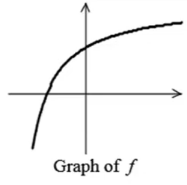
\includegraphics[width=0.3\textwidth]{9.1.1.PNG}
    \end{center}
    \begin{center}
        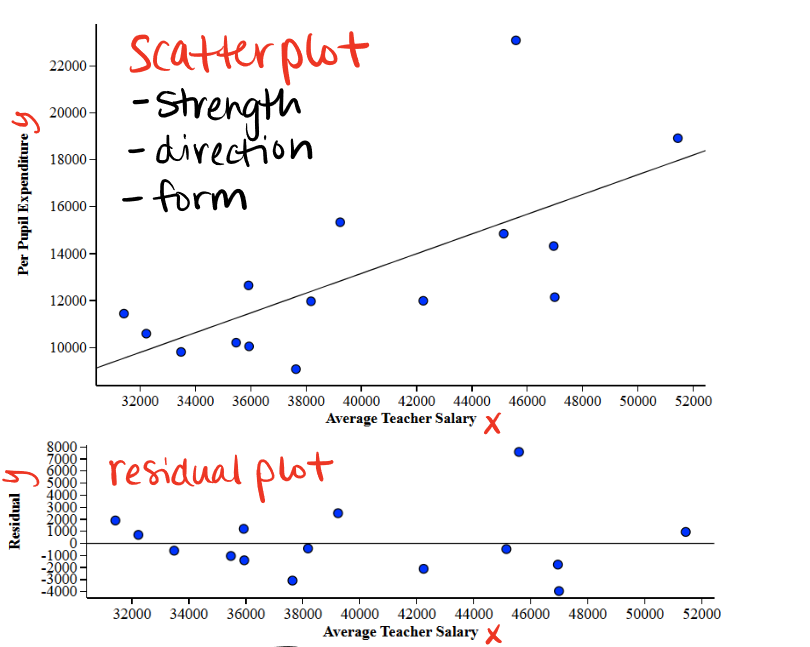
\includegraphics[width=0.8\textwidth]{9.1.2.PNG}
    \end{center}
    \begin{center}
        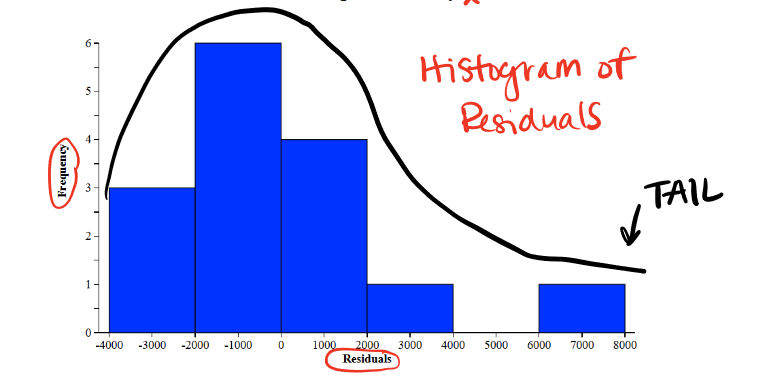
\includegraphics[width=0.8\textwidth]{9.1.3.PNG}
    \end{center}

    Data:
    \begin{itemize}
        \item $n=15$
        \item $r=0.684$
        \item $r^2=0.468$
        \item $s=2865.8$
        \item $s_x=6154.2$
        \item $s_y=3786.1$
        \item $\hat{y}=-3679.1+0.4208x$
    \end{itemize}

    Construct and interpret a 95\% confidence interval for the slope of the population regression line.

    $\beta$ = true population slope between average teacher salary and per pupil expenditure.
    
    \begin{itemize}
        \item Scatterplot shows a moderately positive linear relationship.
        \item $n=15\leq 0.10$(all school districts in the nation)
        \item A histograpm of the residuals appears skewed right. (This is the only condition not correctly met.)
        \item The residual plot shows random scatter around LSRL.
        \item Randomly selected 15 large school districts.
    \end{itemize}

    Linear Regression t-Interval for Slope 

    Using the formula given, we can use invT to get $t^*=2.1604$ and the formula to get the confidence interval $(0.1519, 0.6897)$.

    Calculator Steps:
    \begin{center}
        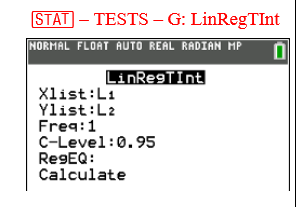
\includegraphics[width=0.4\textwidth]{9.1.4.PNG}
    \end{center}

    We are 95\% confident that the interval from 0.1519 to 0.6897 captures the true slope of the regression line between average teacher salary and per pupil expenditure. However, because our 
    ``Normal Residuals'' condition was not met, we should be careful with this interpretation because it might not be correct.
\end{example}

Most AP Problems will not require you to do what we did in the previous example. Most inference questions come with a computer output, like what is pictured below.
\begin{center}
    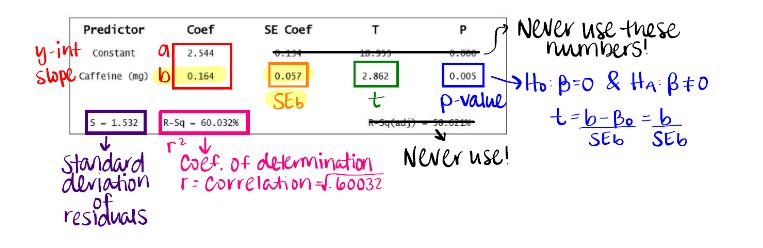
\includegraphics[width=0.8\textwidth]{9.1.5.PNG}
\end{center}

\begin{example}
    A study attempted to establish a linear relationship between IQ score and musical aptitude. The following table is a partial printout of the regression analysis based on a sample of 20 individuals.
    \begin{center}
        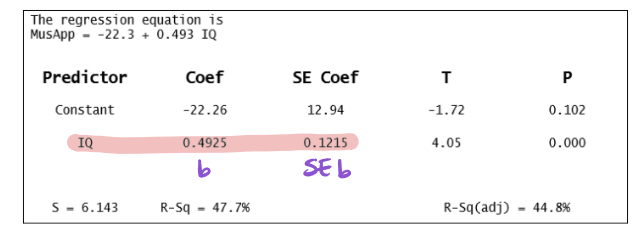
\includegraphics[width=0.8\textwidth]{9.1.6.PNG}
    \end{center}

    Construct and interpret a 99\% confidence interval for the slope of the regression line. Does it suggest a linear relationship? Assume all assumptions and conditions for inference have been met.

    $\beta$ = true population slope between IQ score and musical aptitude

    All assumptions and conditions met 

    Linear Regression t-Interval for Slope 

    $t^*$ = invT(area = .995, df = 18) = 2.8784

    $0.4925\pm 2.8784(0.1215) = (0.1428, 0.8422)$

    We are 99\% confident that the interval from 0.1428 to 0.8422 captures the true slope of the regression line between IQ score and musical aptitude.
\end{example}

\section{Significance Test for a Slope}
\begin{itemize}
    \item The significance test for a slope is called a Linear Regression t-Test for Slope.
    \item It can help us answer three different questions with the hypotheses 
\end{itemize}

Is the relationship between the explanatory and response variable negative?
\begin{itemize}
    \item $H_0: \beta = 0$
    \item $H_A: \beta<0$
\end{itemize}

Is there a relationship between the explanatory and response variable?
\begin{itemize}
    \item $H_0:\beta=0$
    \item $H_A:\beta\neq 0$
\end{itemize}

Is the relationship between the explanatory and response variable positive?
\begin{itemize}
    \item $H_0:\beta=0$
    \item $H_A:\beta>0$
\end{itemize}

Conditions for Regression Inference: Same for the confidence interval 

The test statistics is $t=\frac{\text{statistic-parameter}}{\text{standard error}}$, or $\frac{b}{SE_b}$, where $SE_b=\frac{s}{s_x\sqrt{n-1}}$.

df = n-2, p- value is calculated using your calculator, in the direction of the alternative hypothesis. p-value = tcdf(lower, upper, df)

\begin{itemize}
    \item In your conclusion, you would state the results of your significance test (reject or fail to reject) and then interpret the findings in context 
    \item Note: Having a low p-value and finding evidence of the alternative hypothesis of some linear association does not mean that the association is strong 
\end{itemize}

\begin{example}
    A school counselor is concerned that the number of hours of sleep his students get each night is affecting their GPA in a negative way. He selects a random sample of 14 seniors in his district and asks them how many hours of sleep they get on a typical school night. 
    He then uses school records to determine the most recent grade-point average (GPA) for each student. His data are given below.

    \begin{center}
        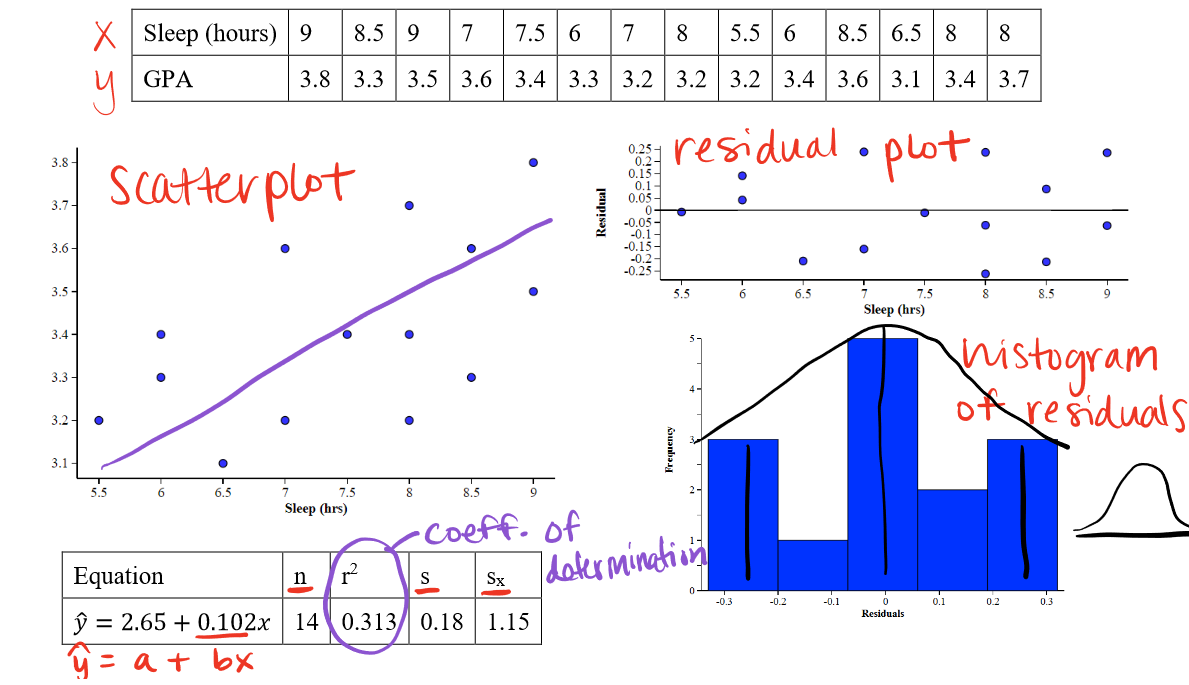
\includegraphics[width=0.8\textwidth]{9.2.1.PNG}
    \end{center}

    Do these data provide convincing evidence, at the 0.05 significance level, of a positive linear relationship between the hours of sleep students typically get and their academic performance?

    $\beta$ = true pop. slope between hours of sleep students typically get and their GPA.

    $H_0: \beta = 0$, $H_A: \beta >0$

    \begin{itemize}
        \item Scatterplot shows a weak positive linear relationship.
        \item $n=14\leq 0.10$(all HS Seniors)
        \item Histogram of residuals doesn't appear normal but no strong skew or outliers 
        \item Residual plot shows random scatter 
        \item Random sample of 14 HS seniors
    \end{itemize}

    Linear Regression t-Test for Slope 

    $t=\frac{0.102}{\frac{0.18}{1.15\sqrt{13}}}=2.3496$, tcdf with this gives $p=0.0184$.

    You can also run this on the calculator 
    \begin{center}
        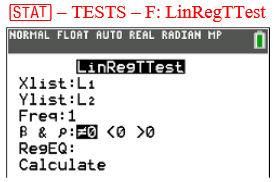
\includegraphics[width=0.4\textwidth]{9.2.2.PNG}
    \end{center}

    Since the p-value of 0.0184 is less than $\alpha = 0.05$, we reject the null. There is convincing evidence of a positive linear relationship between hours of sleep per night and GPA for HS seniors.
\end{example}

\begin{example}
    The computer output given shows a regression analysis of an honors social science course (score in points) versus a reading comprehension score (in points) for 25 sophomores at your school.
    \begin{center}
        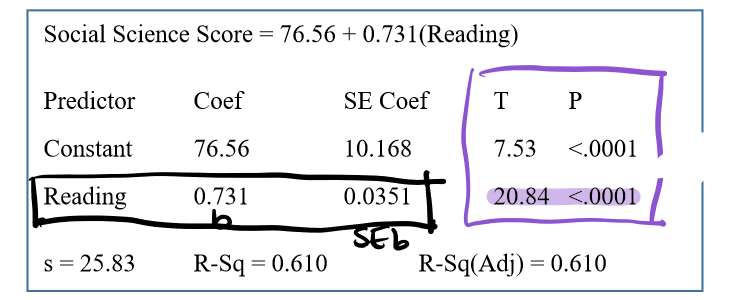
\includegraphics[width=0.8\textwidth]{9.2.3.PNG}
    \end{center}
    Carry out a hypothesis test for these data to determine if there is a linear relationship and interpret your results in the context of the problem. Assume all assumptions and conditions for inference have been met.

    $\beta$ = true pop. slope between social science score and reading score. 

    $H_0:\beta = 0$, $H_A:\beta\neq 0$

    Linear Regression t-Test for Slope

    $t=\frac{0.731}{0.0351}=20.8262$, tcdf with this gives $p\approx 0\times 2 \approx 0$.

    Since the p-value of approx. 0 is less than $\alpha = 0.05$, we reject the null. There is convincing evidence of a linear relationship between social science score and reading score for your school's sophomores.
\end{example}


\end{document}